\chapter{Results}
\label{ch:results}

\section{Introduction}

\section{Simulations and Uncertainties}

\subsection{Simulations on Global Properties}
Interpretation of Global Fractal Dimension
Scale-free GRF vs GRF with Scale

\subsection{Simulations on Local Properties}

\subsection{Error estimates}

Errors for perimeter and area are estimated via the method are on average 1.60\% each. Results for one of the run can be seen in Figure \ref{fig:uncertainties}.

\begin{figure}[t]
    \centering
    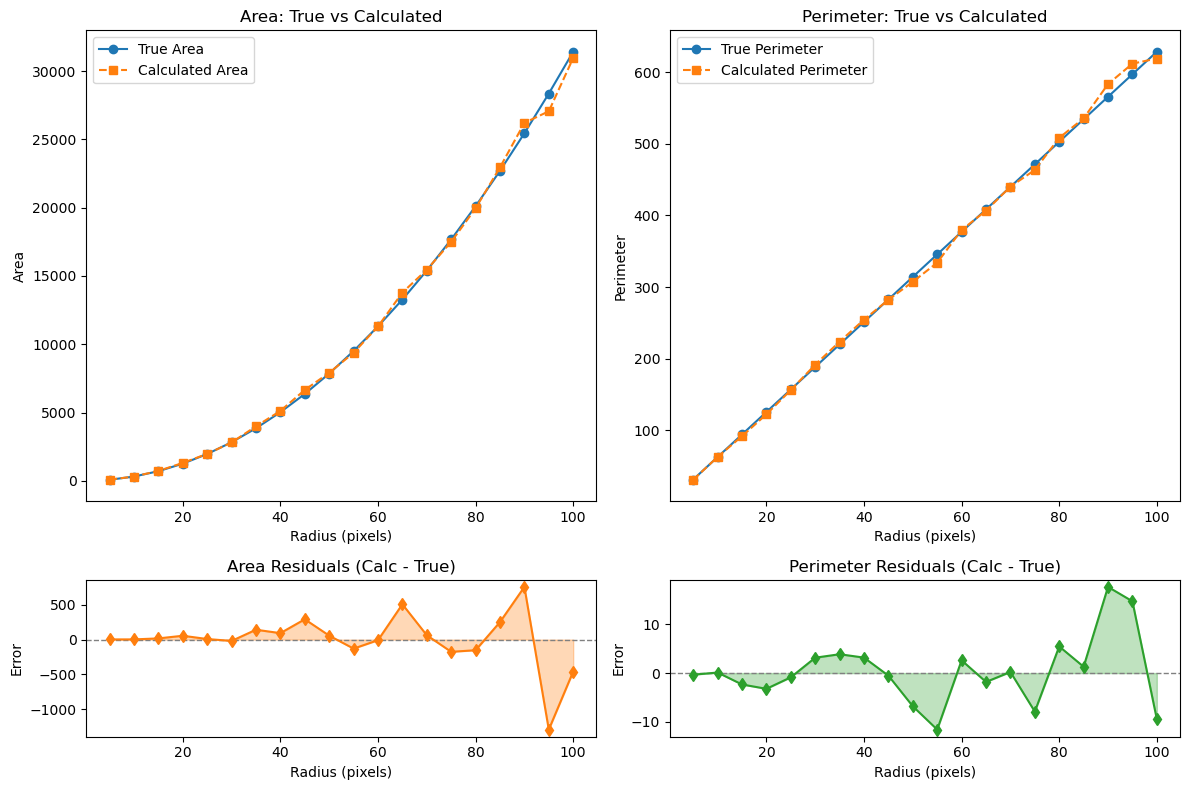
\includegraphics[width=0.75\textwidth]{figures/perimeter_area_uncertainties.png}
    \caption{in arbitrary units }
    \label{fig:uncertainties}
\end{figure}

\section{Global Properties}

\subsection{Global Fractal Dimension}

The data is calculated between , in order to avoid low resolution and straight lines at low column densities and low pixel count at high column densities.
Orion A

\begin{figure}[t]
    \centering
    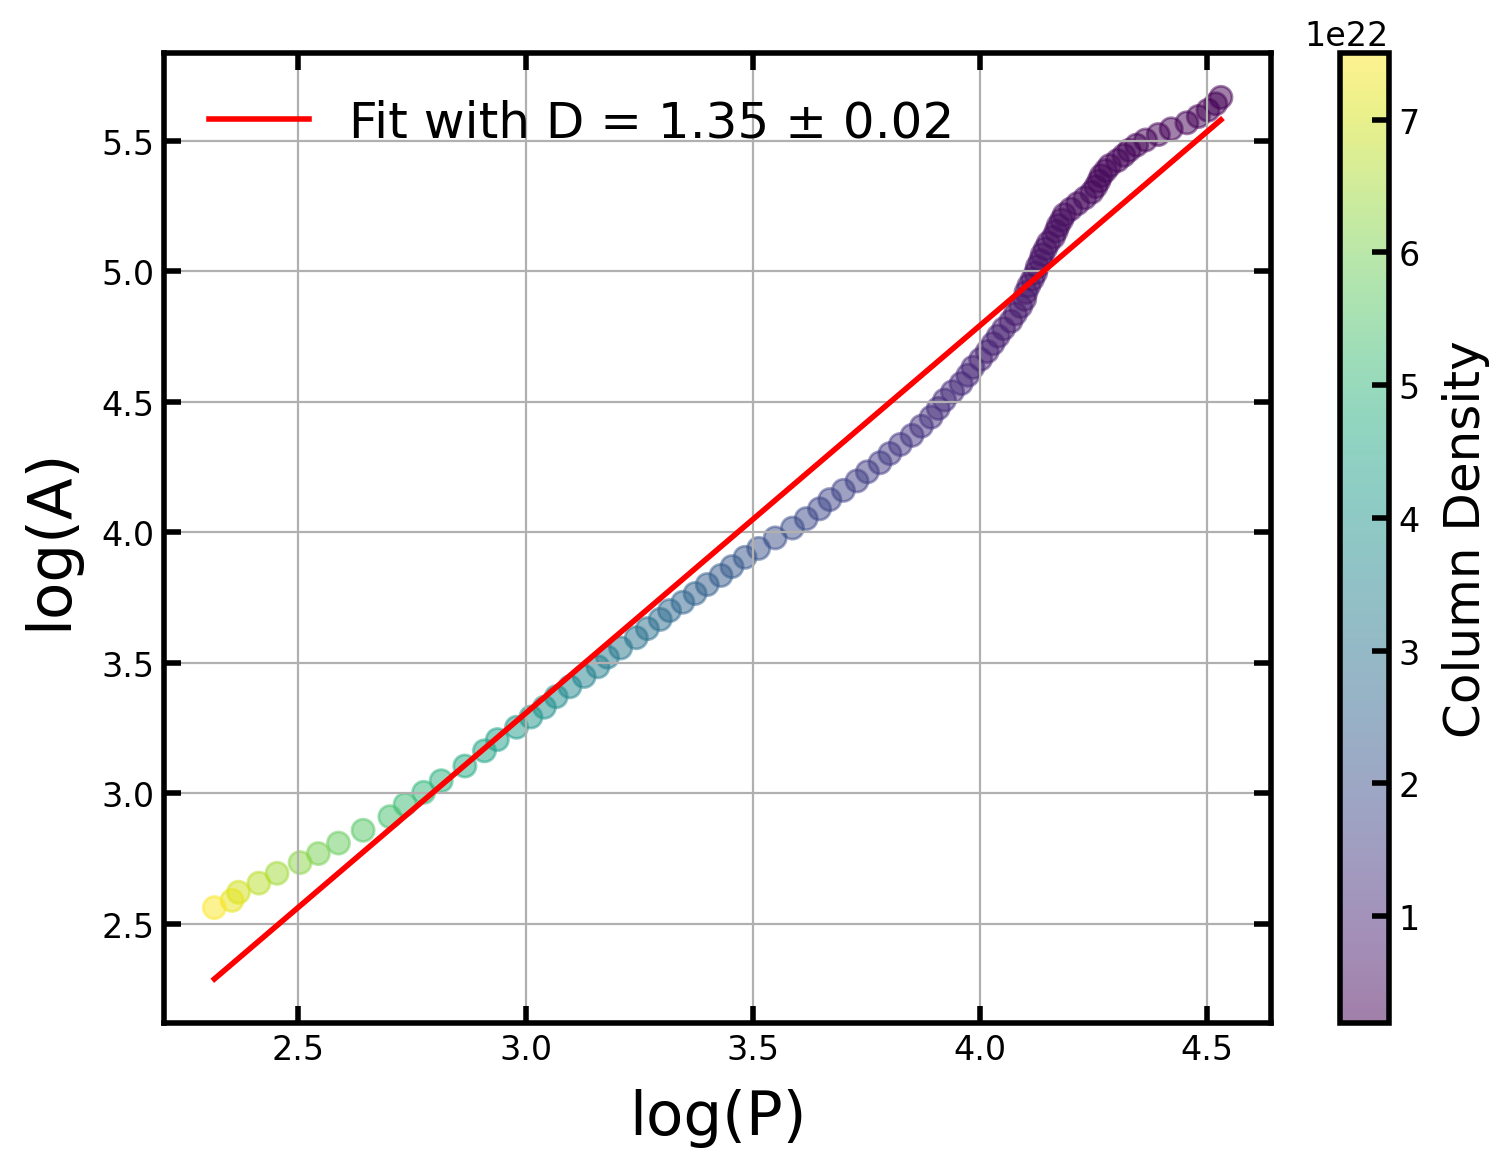
\includegraphics[width=0.5\textwidth]{figures/orion_A_global.png}
    \caption{}
    \label{fig:orion_A_global}
\end{figure}

Orion A double fit

\begin{figure}[t]
    \centering
    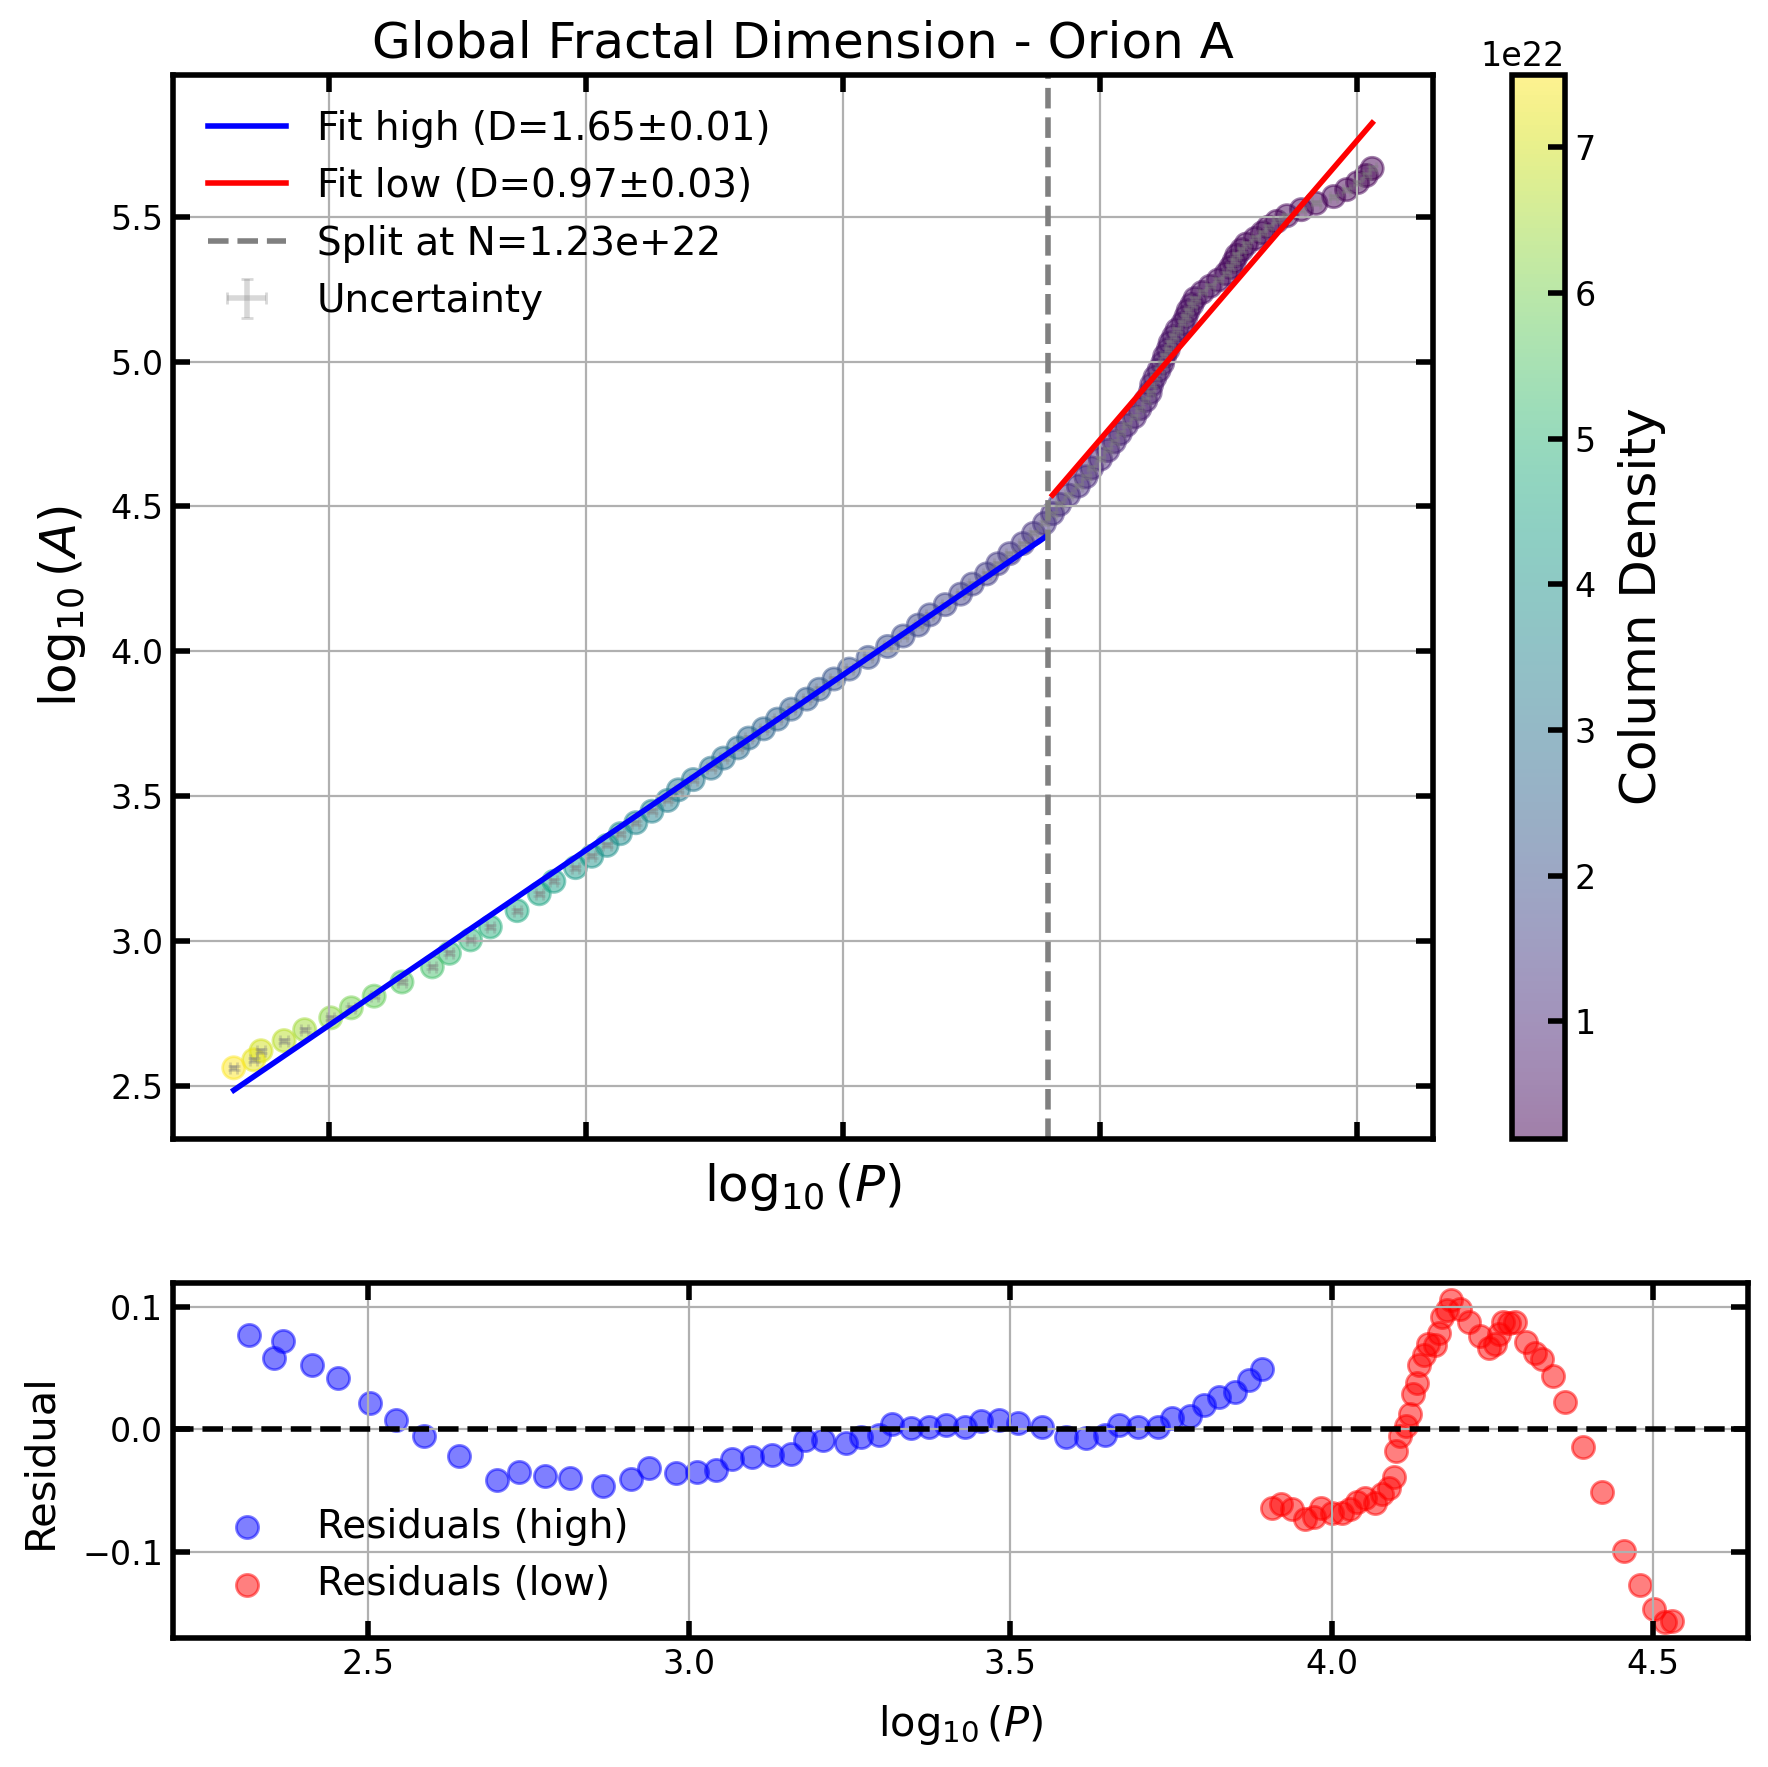
\includegraphics[width=0.5\textwidth]{figures/orion_A_global_double_fit.png}
    \caption{}
    \label{fig:orion_A_global_double_fit}
\end{figure}

Orion B

\begin{figure}[t]
    \centering
    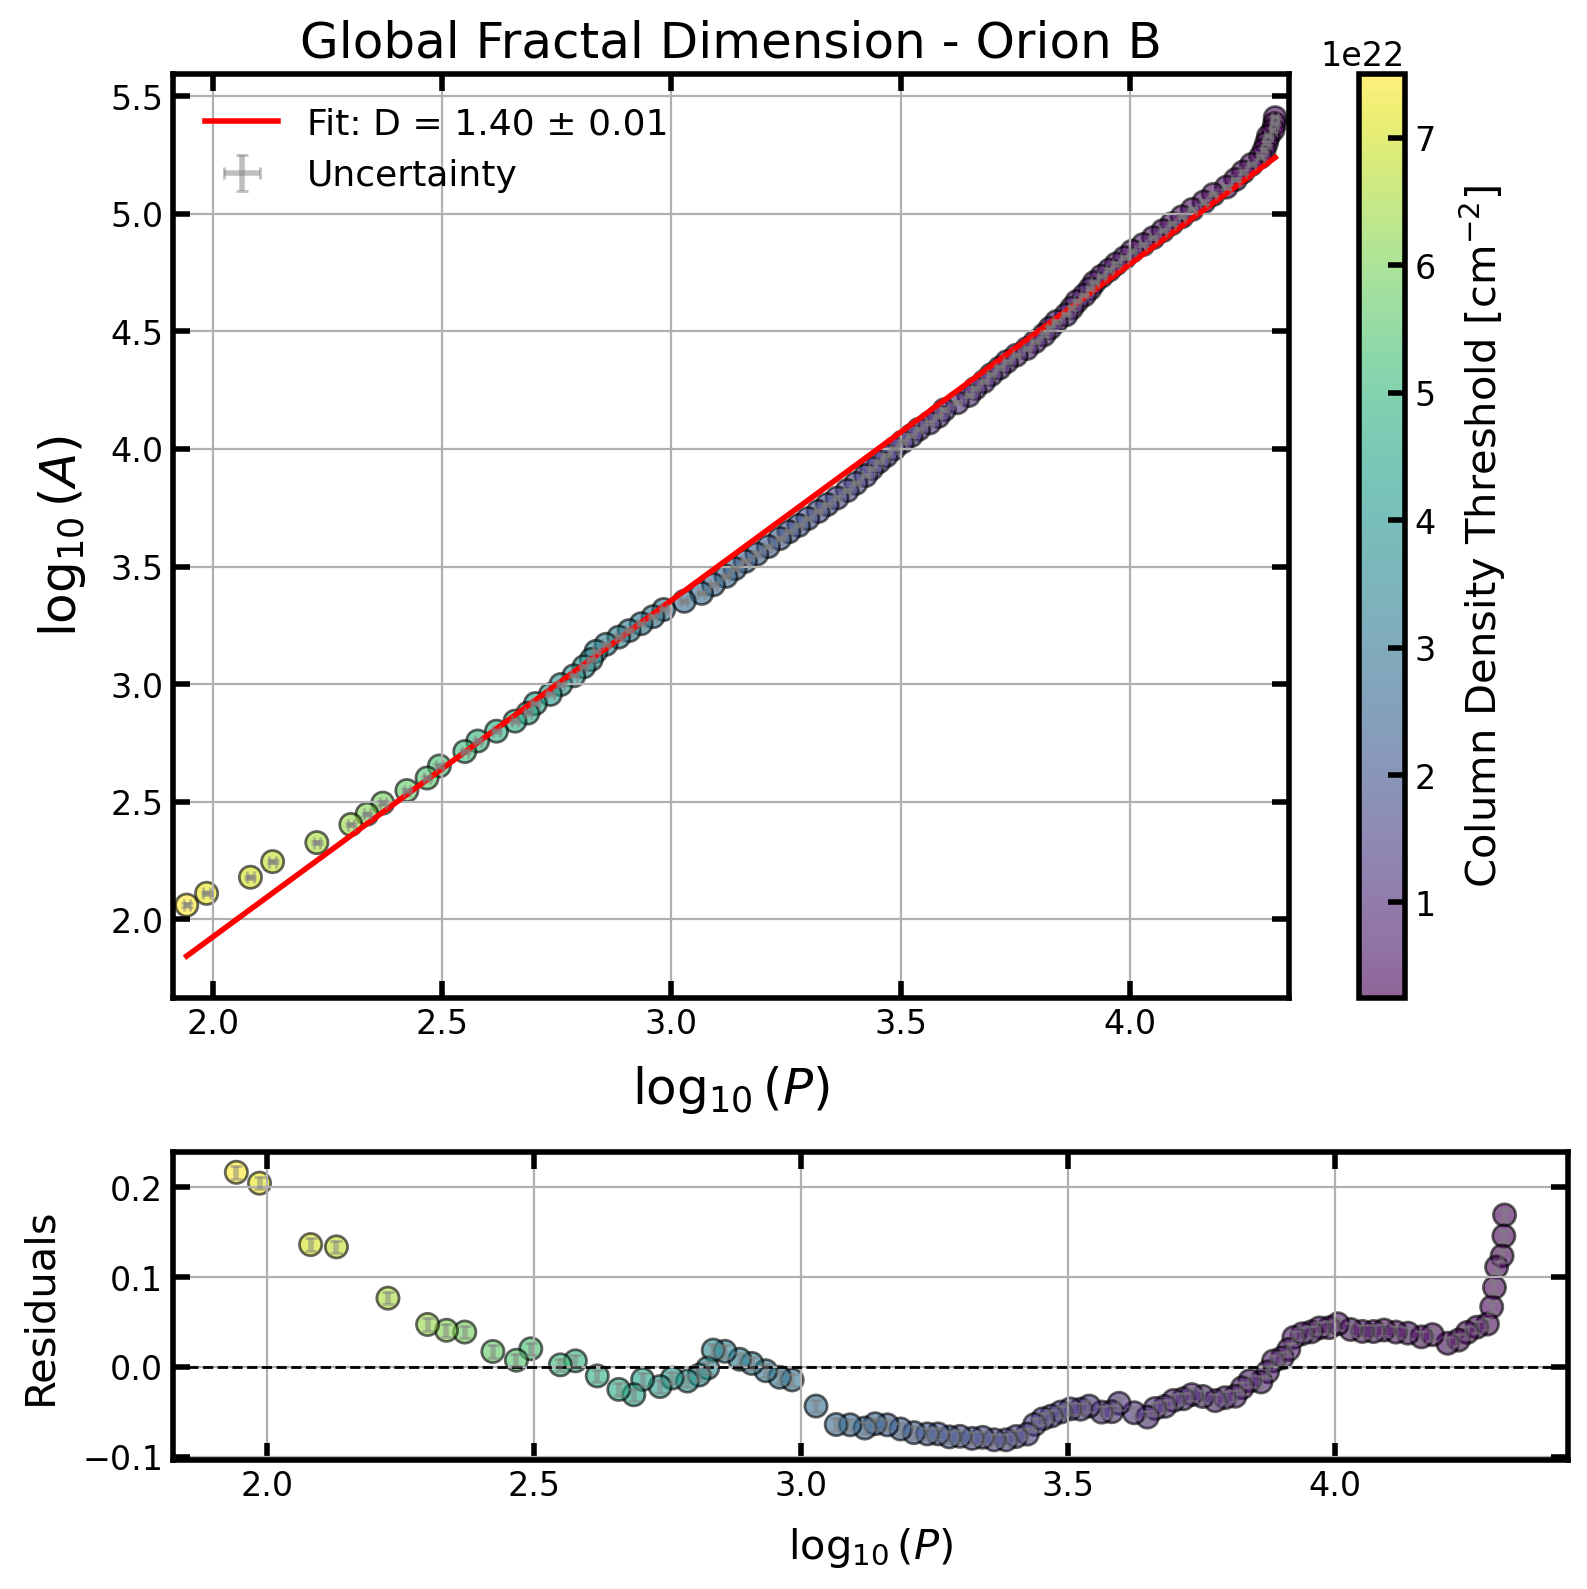
\includegraphics[width=0.5\textwidth]{figures/orion_B_global.png}
    \caption{}
    \label{fig:orion_B}
\end{figure}

The uncertainty from P and A are taken to be 1.6\% via the 
The uncertainties are calculated from the fit routine, since the 

\section{Local Properties}

\subsection{Local Fractal Dimension}

Data Orion A and Orion B

Single structures

\subsection{MSD Plane}

\subsection{Euler Characteristic}

\section{Star Formation}

